\documentclass[tikz,border=2pt]{standalone}
\usepackage{amsmath}
\usepackage{pgfplots}
\pgfplotsset{compat=1.18}

\begin{document}
% A tagged Riemann sum of f(x)=x^2/2+1 on [0,4]: partition 0<1<2<3<4, one tag t_i in each
% subinterval (here the midpoints), rectangle heights f(t_i).
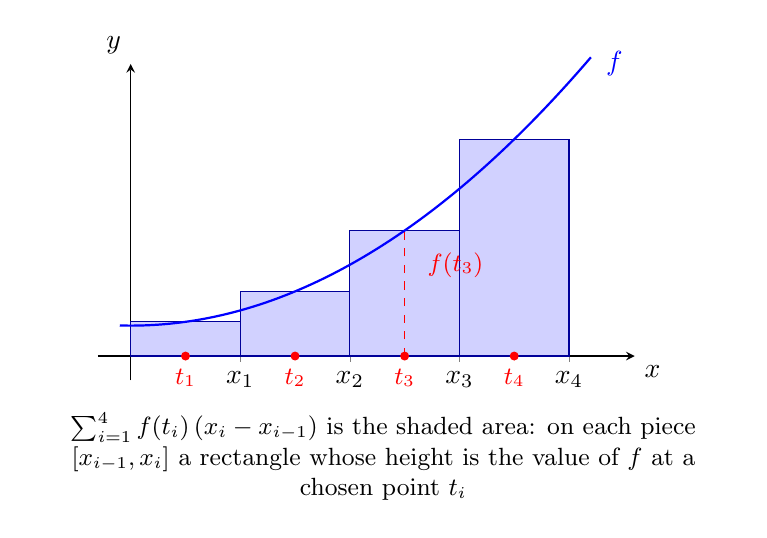
\begin{tikzpicture}
	\begin{axis}[
		axis lines=middle,
		xmin=-0.3, xmax=4.6,
		ymin=-0.8, ymax=9.6,
		xtick={0,1,2,3,4}, xticklabels={$x_0$,$x_1$,$x_2$,$x_3$,$x_4$},
		ytick=\empty,
		xlabel={$x$}, ylabel={$y$},
		xlabel style={below right}, ylabel style={above left},
		samples=100, smooth, clip=false,
		width=8.4cm, height=5.6cm
		]
		% rectangles: height f(midpoint) = 1.125, 2.125, 4.125, 7.125
		\fill[blue!18, draw=blue!60!black] (axis cs:0,0) rectangle (axis cs:1,1.125);
		\fill[blue!18, draw=blue!60!black] (axis cs:1,0) rectangle (axis cs:2,2.125);
		\fill[blue!18, draw=blue!60!black] (axis cs:2,0) rectangle (axis cs:3,4.125);
		\fill[blue!18, draw=blue!60!black] (axis cs:3,0) rectangle (axis cs:4,7.125);
		\addplot[thick, blue, domain=-0.1:4.2] {x^2/2+1};
		\node[blue, anchor=west] at (axis cs:4.25,9.6) {$f$};
		% tags
		\foreach \t in {0.5,1.5,2.5,3.5} {
			\addplot[only marks, mark=*, mark size=1.4pt, red] coordinates {(\t,0)};
		}
		\node[red, anchor=north, font=\small] at (axis cs:0.5,-0.1) {$t_1$};
		\node[red, anchor=north, font=\small] at (axis cs:1.5,-0.1) {$t_2$};
		\node[red, anchor=north, font=\small] at (axis cs:2.5,-0.1) {$t_3$};
		\node[red, anchor=north, font=\small] at (axis cs:3.5,-0.1) {$t_4$};
		\draw[dashed, red] (axis cs:2.5,0) -- (axis cs:2.5,4.125);
		\node[red, anchor=west, font=\small] at (axis cs:2.62,3.0) {$f(t_3)$};
	\end{axis}
	\node[anchor=north, font=\small, align=flush center, text width=8.8cm] at ([yshift=-2pt]current axis.outer south) {$\sum_{i=1}^{4}f(t_i)\,(x_i-x_{i-1})$ is the shaded area: on each piece $[x_{i-1},x_i]$ a rectangle whose height is the value of $f$ at a chosen point $t_i$};
\end{tikzpicture}
\end{document}
